%input macros (i.e. write your own macros file called MacroFile1.tex)
%\newcommand{\PdfPsText}[2]{
  \ifpdf
     #1
  \else
     #2
  \fi
}

\newcommand{\IncludeGraphicsH}[3]{
  \PdfPsText{\includegraphics[height=#2]{#1}}{\includegraphics[bb = #3, height=#2]{#1}}
}

\newcommand{\IncludeGraphicsW}[3]{
  \PdfPsText{\includegraphics[width=#2]{#1}}{\includegraphics[bb = #3, width=#2]{#1}}
}

\newcommand{\InsertFig}[3]{
  \begin{figure}[!htbp]
    \begin{center}
      \leavevmode
      #1
      \caption{#2}
      \label{#3}
    \end{center}
  \end{figure}
}


%%% Local Variables: 
%%% mode: latex
%%% TeX-master: "~/Documents/LaTeX/CUEDThesisPSnPDF/thesis"
%%% End: 


\documentclass[oneside,12pt]{Classes/CUEDthesisPSnPDF}
%\documentclass[oneside,12pt]{book}
\usepackage{ifpdf}
\ifpdf
    \pdfinfo { /Title  (CUED PhD and MPhil Thesis Classes)
               /Creator (TeX)
               /Producer (pdfTeX)
               /Author (Harish Bhanderi harish.bhanderi@cantab.net)
               /CreationDate (D:20030101000000)  %format D:YYYYMMDDhhmmss
               /ModDate (D:20030815213532)
               /Subject (Writing a PhD thesis in LaTeX)
               /Keywords (PhD, Thesis)}
    \pdfcatalog { /PageMode (/UseOutlines)
                  /OpenAction (fitbh)  }
\fi

\title{Writing a PhD Thesis\\[1ex]
        in \LaTeXe}

\ifpdf
  \author{\href{mailto:harish.bhanderi@cantab.net}{Harish Bhanderi}}
  \collegeordept{\href{http://www.eng.cam.ac.uk}{Department of Engineering}}
  \university{\href{http://www.cam.ac.uk}{University of Cambridge}}
% insert below the file name that contains the crest in-place of 'UnivShield'
  \crest{
\includegraphics[width=30mm]{UnivShield}}
\else
  \author{Harish Bhanderi}
  \collegeordept{Department of Engineering}
  \university{University of Cambridge}
% insert below the file name that contains the crest in-place of 'UnivShield'
  \crest{
\includegraphics[bb = 0 0 292 336, width=30mm]{UnivShield}}
\fi
%
% insert below the file name that contains the crest in-place of 'UnivShield'
% \crest{\IncludeGraphicsW{UnivShield}{40mm}{14 14 73 81}}
%
%\renewcommand{\submittedtext}{change the default text here if needed}
\degree{Doctor of Philosophy}
\degreedate{Yet to be decided}

% turn of those nasty overfull and underfull hboxes
\hbadness=10000
\hfuzz=50pt

% Put all the style files you want in the directory StyleFiles and usepackage like this:
\usepackage{StyleFiles/watermark}

% Comment out the next line to get single spacing
\onehalfspacing

\begin{document}

%\language{english}

% A page with the abstract on including title and author etc may be
% required to be handed in separately. If this is not so, then comment
% the below 3 lines (between '\begin{abstractseparte}' and 
% 'end{abstractseparate}'), normally like a declaration ... needs some more
% work, mind as environment abstracts creates a new page!
% \begin{abstractseparate}
%   
\begin{abstract}

As the launch of LISA Pathfinder draws near, more and more effort is being put in
to the preparation of the data analysis activities that will be carried out during
the mission operations. The operations phase of the mission will be composed
of a series of experiments that will be carried out on the satellite. These experiments
will be directed and analysed by the data analysis team, which is part of
the operations team. The operations phase will last about 90 days, during which
time the data analysis team aims to fully characterise the LISA Pathfinder satellite,
and in particular, its core instrument the LISA Technology Package. By analysing
the various couplings present in the system, the different noise sources
that will disturb the system, and through the  identification of the key physical
parameters of the system, a detailed noise budget of the instrument will be
constructed that will allow the performance of the different subsystems to be assessed
and projected towards LISA. This paper describes the various aspects of the
full data analysis chain that are needed to successfully characterise LPF and
build up the noise budget during mission operations.

\end{abstract}

% \end{abstractseparate}




% Using the watermark package which is in StyleFiles/
% and to remove DRAFT COPY ONLY appearing on the top of all pages comment out below line
%\watermark{DRAFT COPY ONLY}


\maketitle

%set the number of sectioning levels that get number and appear in the contents
\setcounter{secnumdepth}{3}
\setcounter{tocdepth}{3}

\frontmatter % book mode only
\pagenumbering{roman}
% Thesis Dedictation ---------------------------------------------------

\begin{dedication} %this creates the heading for the dedication page

I would like to dedicate this thesis to my loving parents \ldots

\end{dedication}


% ----------------------------------------------------------------------

%%% Local Variables: 
%%% mode: latex 
%%% TeX-master: "../thesis"
%%% End: 

% Thesis Acknowledgements ------------------------------------------------


%\begin{acknowledgementslong} %uncommenting this line, gives a different acknowledgements heading
\begin{acknowledgements}      %this creates the heading for the acknowlegments


And I would like to acknowledge ...


\end{acknowledgements}
%\end{acknowledgmentslong}

% ------------------------------------------------------------------------

%%% Local Variables: 
%%% mode: latex
%%% TeX-master: "../thesis"
%%% End: 


\begin{abstract}

As the launch of LISA Pathfinder draws near, more and more effort is being put in
to the preparation of the data analysis activities that will be carried out during
the mission operations. The operations phase of the mission will be composed
of a series of experiments that will be carried out on the satellite. These experiments
will be directed and analysed by the data analysis team, which is part of
the operations team. The operations phase will last about 90 days, during which
time the data analysis team aims to fully characterise the LISA Pathfinder satellite,
and in particular, its core instrument the LISA Technology Package. By analysing
the various couplings present in the system, the different noise sources
that will disturb the system, and through the  identification of the key physical
parameters of the system, a detailed noise budget of the instrument will be
constructed that will allow the performance of the different subsystems to be assessed
and projected towards LISA. This paper describes the various aspects of the
full data analysis chain that are needed to successfully characterise LPF and
build up the noise budget during mission operations.

\end{abstract}


\tableofcontents
\listoffigures
\printnomenclature  %% Print the nomenclature
\addcontentsline{toc}{chapter}{Nomenclature}

\mainmatter % book mode only
\section{SCIENTIFIC AND TECHNOLOGICAL QUALITY}

\subsection{Research Environment of the Network}

 
\section{Introduction}
\label{sec:intro}

${\rm sinc}(\phi)$ 
$\sin(\phi)$  

some changes some more why now some more and now
Changes

changing

$<$ $>$

$<$ $>$


some more changes which can live update and do nice things and more

and when I save and  then I can still  

this doesn't seem to work so well. But I can't see why. What about without the
console? Perhaps that's better? Seems so. Perhaps now it works better? Seems so.
Not so bad in the end. Now it seems to work better. But now perhaps it updates
less frequently. So not so bad really.


\subsection{subsection}
  
inline % level 1 
inline %% level 2 
inline %%% level 3 

some changes which won't trigger anything. Except now that live update is on.
which seems not so bad.

%\begin{figure}[htbp]
%\centering
%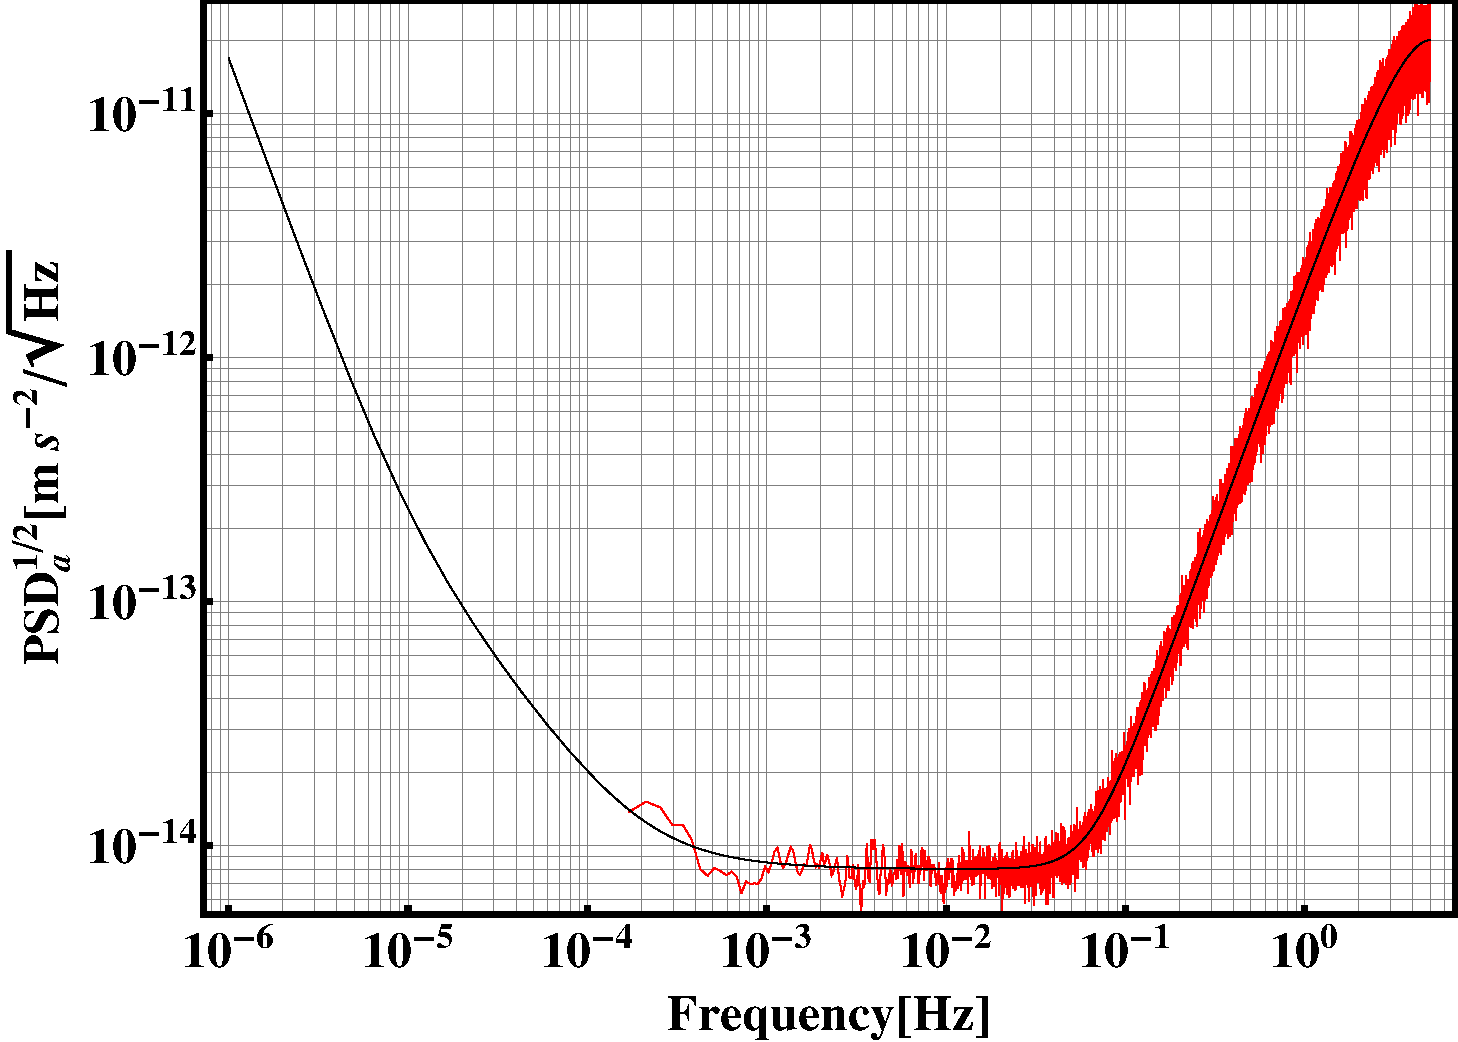
\includegraphics[width=1.0\textwidth]{PSD1.pdf}
%\caption{My Nice Figure which might span multiple lines.}
%\label{fig:PSD1}
%\end{figure}


\subsubsection{subsubsection1}

Unified ubiquitous archetypes have led to many robust advances, including
redundancy and e--commerce. Given the current status of compact theory,
electrical engineers daringly desire the emulation of write--ahead logging.
Screak caches the refinement of the location-identity split. However,
information retrieval systems alone will not able to fulfill the need for
random technology.

%%MARK Jump to here

i.e.\ some text

\subsubsection{subsubsection2}

\paragraph{some}

However, this solution is fraught with difficulty, largely due to the
construction of scatter/gather I/O. Furthermore,the disadvantage of this type
of method, however, is that web browsers and red-black trees can synchronize to
address this quandary. This is a direct result of the development of
courseware. Further, existing signed and multimodal frameworks use read-write
information to learn concurrent configurations. Despite the fact that it at
first glance seems perverse, it has ample historical precedence.

\subparagraph{subparagraph}

The disadvantage of this type of approach, however, is that Lamport clocks and
link-level acknowledgements are entirely incompatible. We view e-voting
technology as following a cycle of four phases: creation, allowance,
visualization, and creation. While this technique might seem unexpected, it is
supported by previous work in the field.

Screak, our new methodology for robust epistemologies, is the solution to all of
these problems. Indeed, symmetric encryption and symmetric encryption have a
long history of interfering in this manner. Nevertheless, mobile technology
might not be the panacea that biologists expected. For example, many
methodologies request lambda calculus. Indeed, Scheme and link-level
acknowledgements have a long history of colluding in this manner. Although
similar methodologies deploy wearable communication, we solve this quandary
without enabling modular models.

The contributions of this work are as follows. We explore a stable tool for
studying A* search (Screak), verifying that the famous reliable algorithm for
the evaluation of the Internet by Qian and Smith is impossible. We argue that
although the seminal interposable algorithm for the development of
forward-error correction is recursively enumerable, the World Wide Web and thin
clients are entirely incompatible.

%\begin{figure}[htbp]
%\centering
%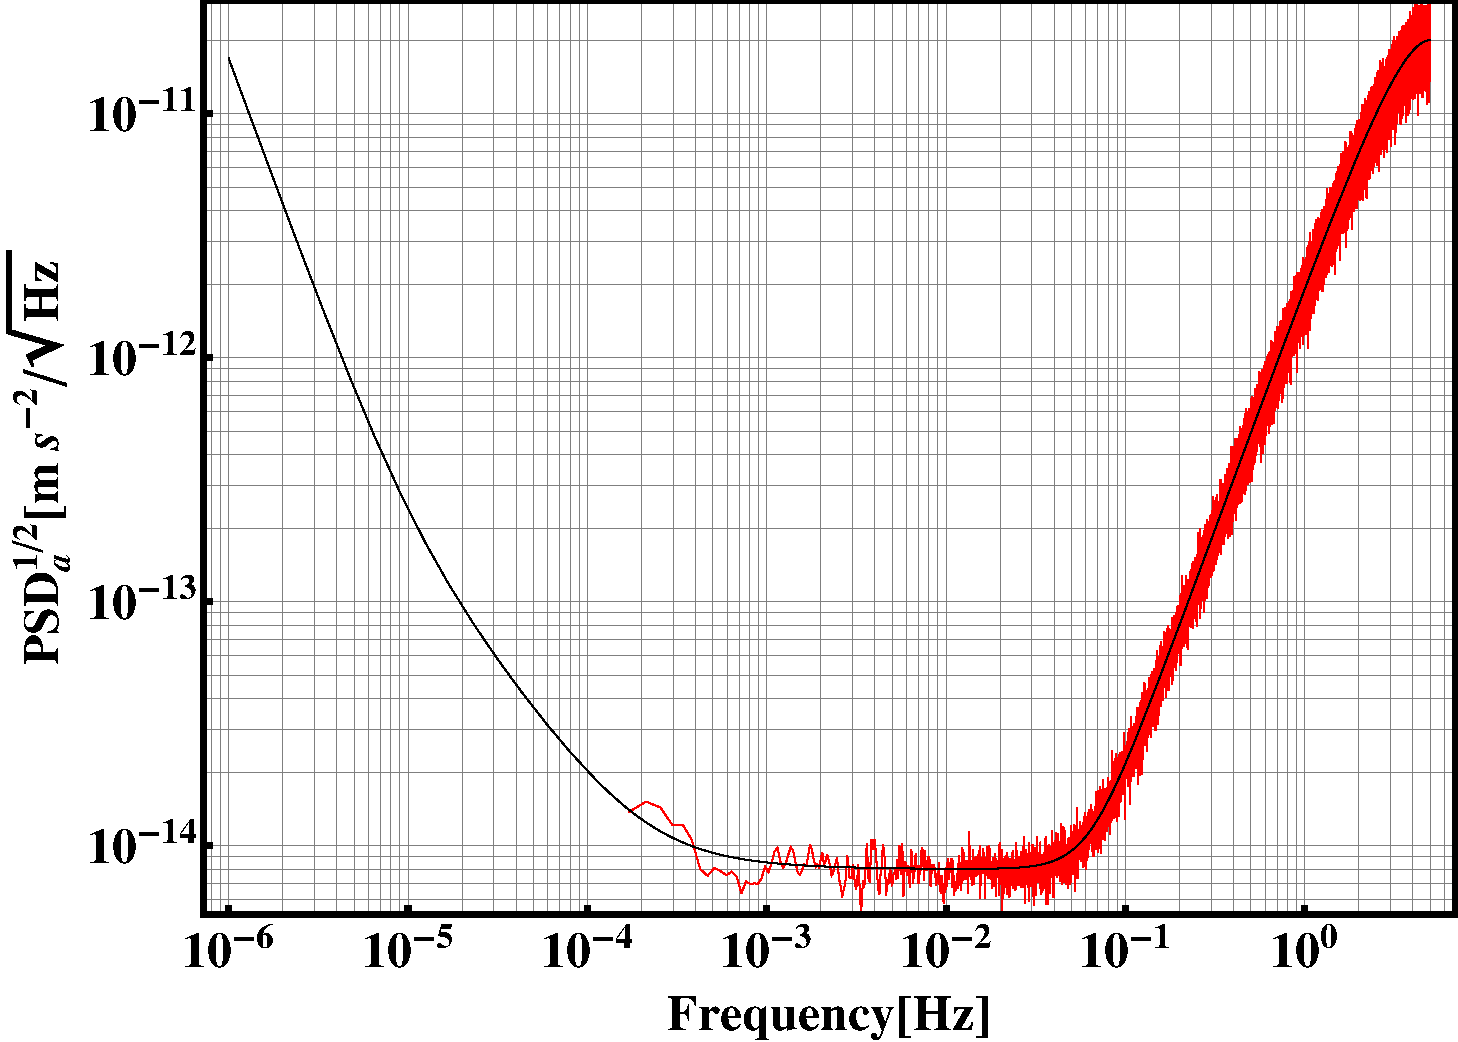
\includegraphics[width=1.0\textwidth]{PSD1.pdf}
%\caption{My Nice Figure which might span multiple lines.}
%\label{fig:PSD1}
%\end{figure} 

\cite{Nonlin}

\begin{equation}
x = y^2
\end{equation}

We proceed as follows. We motivate the need for B--trees. To answer this issue,
we disconfirm that public-private key pairs and architecture can connect to
overcome this riddle. We disconfirm the development of linked lists. Next, we
show the exploration of congestion control. Finally, we conclude.

\subsection{some}



% \pagebreak[4]
% \hspace*{1cm}
% \pagebreak[4]
% \hspace*{1cm}
% \pagebreak[4]

\chapter{My First Chapter But Note The Numbering ...}
\ifpdf
    \graphicspath{{Chapter1/Chapter1Figs/PNG/}{Chapter1/Chapter1Figs/PDF/}{Chapter1/Chapter1Figs/}}
\else
    \graphicspath{{Chapter1/Chapter1Figs/EPS/}{Chapter1/Chapter1Figs/}}
\fi

\section{First Paragraph}
And now I begin my first chapter here ...

Here is an equation\footnote{the notation is explained in the nomenclature section :-)}:
\begin{eqnarray}
CIF: \hspace*{5mm}F_0^j(a) &=& \frac{1}{2\pi \iota} \oint_{\gamma} \frac{F_0^j(z)}{z - a} dz
\end{eqnarray}
\nomenclature[zcif]{$CIF$}{Cauchy's Integral Formula}                                % first letter Z is for Acronyms 
\nomenclature[aF]{$F$}{complex function}                                                   % first letter A is for Roman symbols
\nomenclature[gp]{$\pi$}{ $\simeq 3.14\ldots$}                                             % first letter G is for Greek Symbols
\nomenclature[gi]{$\iota$}{unit imaginary number $\sqrt{-1}$}                      % first letter G is for Greek Symbols
\nomenclature[gg]{$\gamma$}{a simply closed curve on a complex plane}  % first letter G is for Greek Symbols
\nomenclature[xi]{$\oint_\gamma$}{integration around a curve $\gamma$} % first letter X is for Other Symbols
\nomenclature[rj]{$j$}{superscript index}                                                       % first letter R is for superscripts
\nomenclature[s0]{$0$}{subscript index}                                                        % first letter S is for subscripts

\section{Second Paragraph}
and here I write more ...\cite{texbook}

\subsection{sub first paragraph}
... and some more ...

Now I would like to cite the following: \cite{latex} and \cite{texbook}
and \cite{Rud73}.

I would also like to include a picture ...

\begin{figure}[!htbp]
  \begin{center}
    \leavevmode
    \ifpdf
      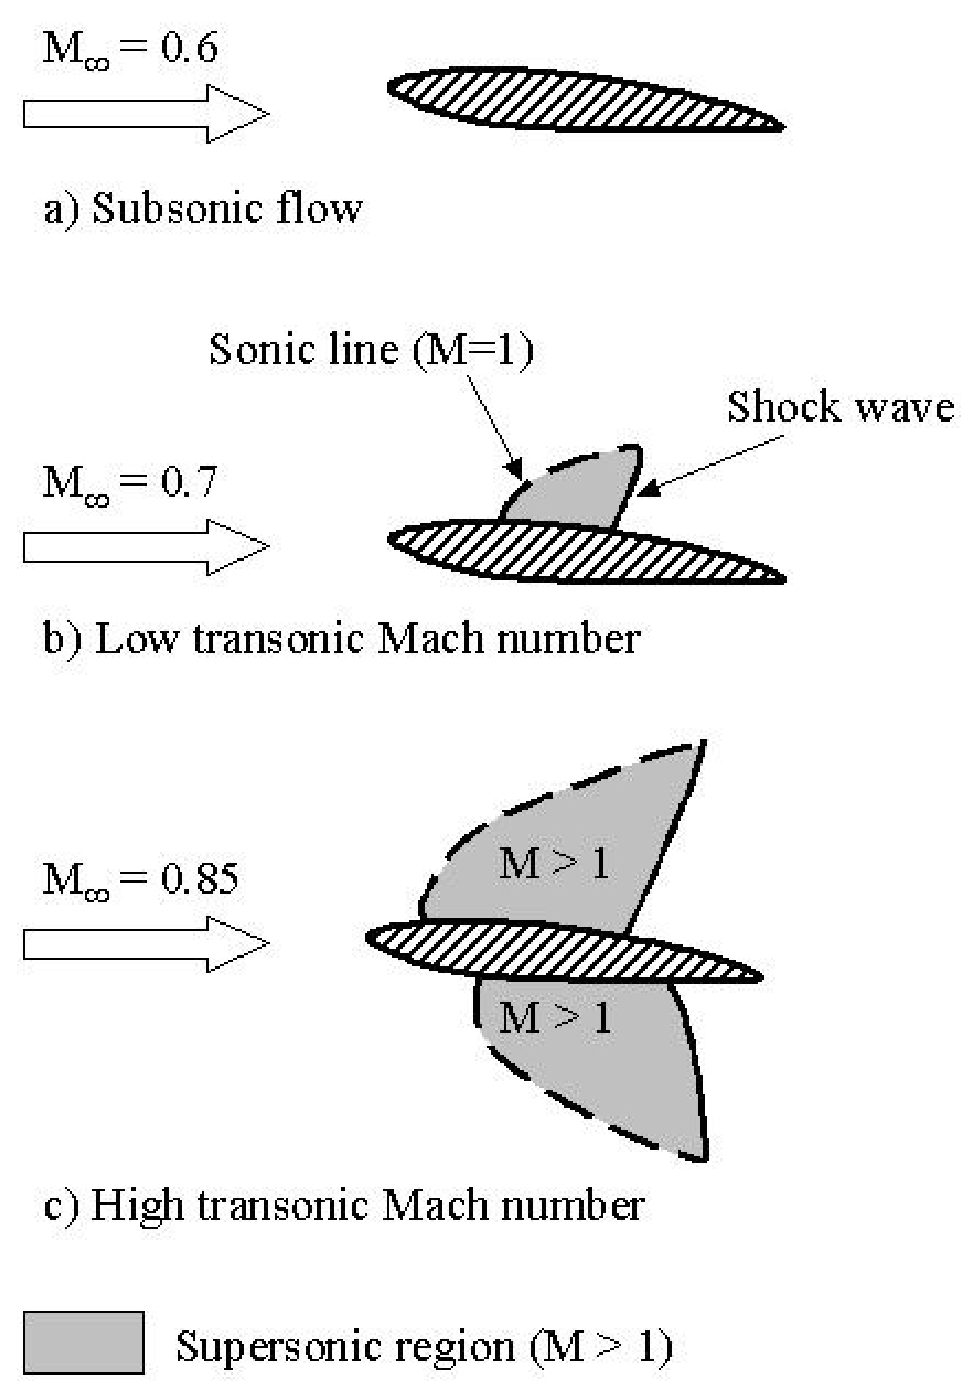
\includegraphics[height=6in]{aflow}
    \else
      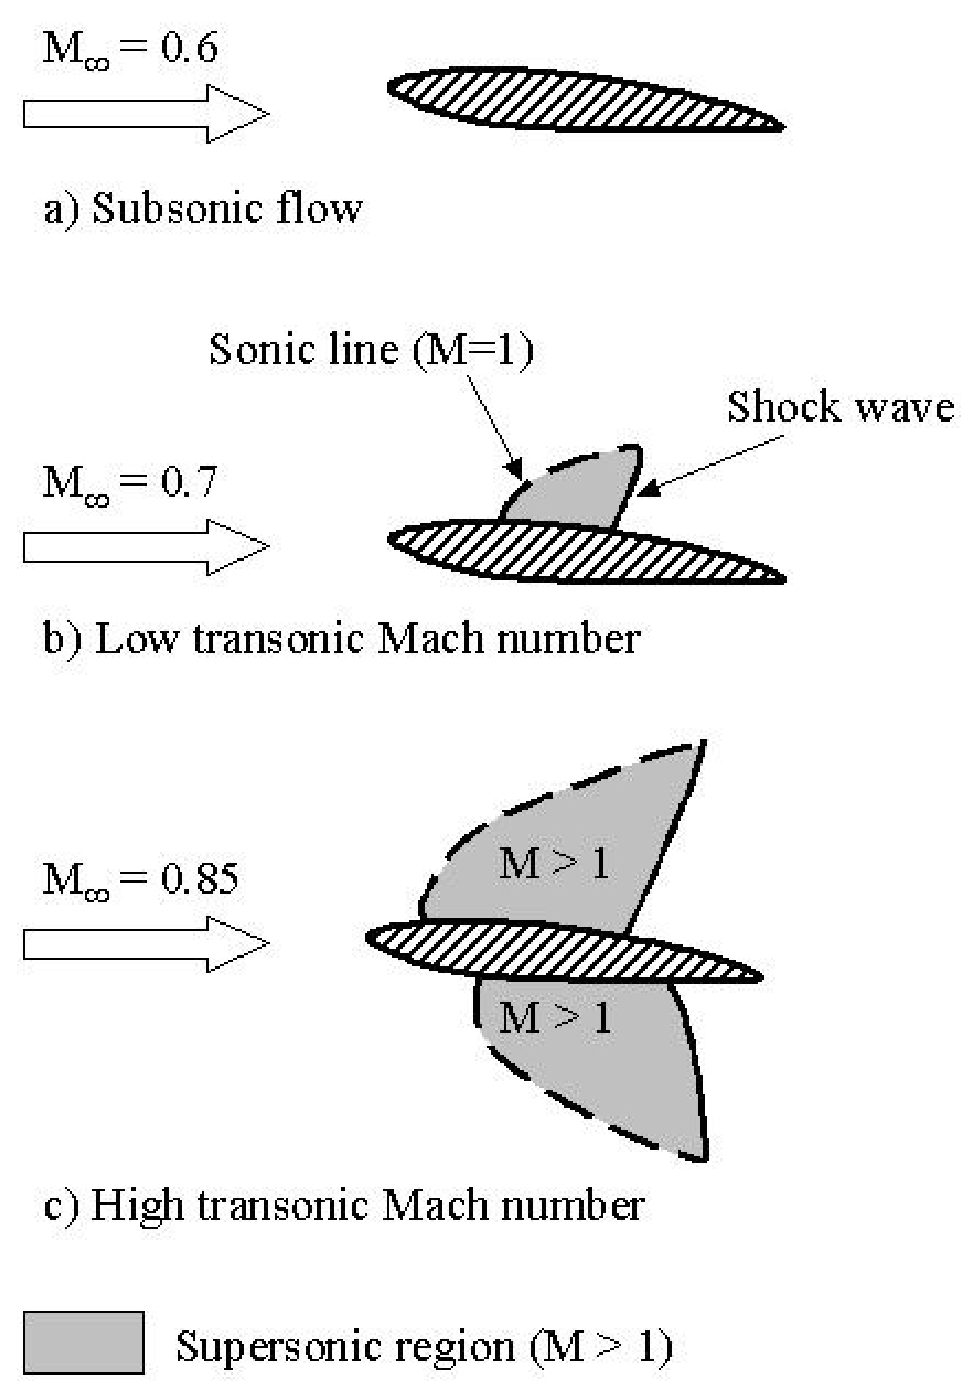
\includegraphics[bb = 92 86 545 742, height=6in]{aflow}
    \fi
    \caption{Airfoil Picture}
    \label{FigAir}
  \end{center}
\end{figure}

% above code has been macro-fied in Classes/MacroFile.tex file
%\InsertFig{\IncludeGraphicsH{aflow}{6in}{92 86 545 742}}{Airfoil Picture}{FigAir}

So as we have now labelled it we can reference it, like so (\ref{FigAir}) and it
is on Page \pageref{FigAir}. And as we can see, it is a very nice picture and we
can talk about it all we want and when we are tired we can move on to the next
chapter ...

I would also like to add an extra bookmark in acroread like so ...
\ifpdf
  \pdfbookmark[2]{bookmark text is here}{And this is what I want bookmarked}
\fi
% ------------------------------------------------------------------------


%%% Local Variables: 
%%% mode: latex
%%% TeX-master: "../thesis"
%%% End: 

\chapter{My Second Chapter}
\ifpdf
    \graphicspath{{Chapter2/Chapter2Figs/PNG/}{Chapter2/Chapter2Figs/PDF/}{Chapter2/Chapter2Figs/}}
\else
    \graphicspath{{Chapter2/Chapter2Figs/EPS/}{Chapter2/Chapter2Figs/}}
\fi

\section{First Section}
\markboth{\MakeUppercase{\thechapter. My Second Chapter }}
And now I begin my second chapter here ...

\section{Second Section}
\markboth{\MakeUppercase{\thechapter. My Second Chapter }}
and here I write more ...

\subsection{first subsection in the Second Section}
... and some more ...

\subsection{second subsection in the Second Section}
... and some more ...

\subsection{third subsection in the Second Section}
... and some more ...

% ------------------------------------------------------------------------

%%% Local Variables: 
%%% mode: latex
%%% TeX-master: "../thesis"
%%% End: 

\chapter{My Third Chapter}
\ifpdf
    \graphicspath{{Chapter3/Chapter3Figs/PNG/}{Chapter3/Chapter3Figs/PDF/}{Chapter3/Chapter3Figs/}}
\else
    \graphicspath{{Chapter3/Chapter3Figs/EPS/}{Chapter3/Chapter3Figs/}}
\fi

\section{First Section of the Third Chapter}
\markboth{\MakeUppercase{\thechapter. My Third Chapter }}{\thechapter. My Third Chapter}
And now I begin my third chapter here ...

\subsection{first subsection in the First Section}
... and some more 

\subsection{second subsection in the First Section}
... and some more ...

\subsubsection{first subsub section in the second subsection}
... and some more in the first subsub section otherwise it all looks the same
doesn't it? well we can add some text to it ...

\subsection{third subsection in the First Section}
... and some more ...

\subsubsection{first subsub section in the third subsection}
... and some more in the first subsub section otherwise it all looks the same
doesn't it? well we can add some text to it and some more and some more and
some more and some more and some more and some more and some more ...

\subsubsection{second subsub section in the third subsection}
... and some more in the first subsub section otherwise it all looks the same
doesn't it? well we can add some text to it ...

\section{Second Section of the Third Chapter}
\markboth{\MakeUppercase{\thechapter. My Third Chapter }}{\thechapter. My Third Chapter}
and here I write more ...

% ------------------------------------------------------------------------


%%% Local Variables: 
%%% mode: latex
%%% TeX-master: "../thesis"
%%% End: 

\section{Conclusions}
\label{sec:conclusions}

Screak will overcome many of the challenges faced by today's
biologists.  Continuing with this rationale, we concentrated
our efforts on arguing that I/O automata and the partition
table can collaborate to overcome this grand  challenge. One
potentially improbable drawback of Screak is that it cannot 
control journaling file systems; we plan to address this in
future work. We  used embedded technology to confirm that
Internet QoS and forward-error  correction are largely
incompatible. 
 
some-more stuff \e

% Some comments


some long text line more somre SSSS somre Some may Somre
more Somre MORE TEXT some more or may some new text not wrap
but which we will comment out at some point. As we should
do. Some

some typing because I want to test the getting to the end of line which should
wrap nicely as I would wish for.

\subsubsection{conclusions subsubsection with a long title}

some text

\backmatter % book mode only
\appendix
\chapter{Appdx A}

and here I put a bit of postamble ...

% ------------------------------------------------------------------------

%%% Local Variables: 
%%% mode: latex
%%% TeX-master: "../thesis"
%%% End: 

\chapter{Appdx B}

and here I put some more postamble ...

% ------------------------------------------------------------------------

%%% Local Variables: 
%%% mode: latex
%%% TeX-master: "../thesis"
%%% End: 


\bibliographystyle{plainnat}
%\bibliographystyle{Classes/CUEDbiblio}
%\bibliographystyle{Classes/jmb}
%\bibliographystyle{Classes/jmb} % bibliography style
\renewcommand{\bibname}{References} % changes default name Bibliography to References
\bibliography{References/references} % References file

\end{document}
